\textbf{Consider the first order linear initial boundary value problem
\begin{align*}
u_t=u_x, ~~~~x\in[-1,1],~~t>0,~~u(\pm 1,t)=u(x,0)=0,
\end{align*}
with initial data $u(x,0) = \exp(-60(x-1/2)^2)$. Write a program to solve this problem by a matrix-based Chebyshev spectral discretization in $x$ coupled with the third order Adams-Bashforth formula in $t$, 
\begin{align*}
u^{(n+3)} = u^{(n+2)}+\frac{1}{12}\Delta t\left(23f^{(n+2)}-16f^{(n+1)}+5f^{(n)}\right).
\end{align*}
Initial values can be supplied from the exact solution. Take $N=50$ and \newline $\Delta t=\nu N^{-2}$, where $\nu$ is a parameter. For each of the two choices $\nu = 7$ and $\nu = 8$, produce one plot of the computed solution at $t=1$ and another that superimposes the stability region in the $\lambda\Delta t$-plane, the eigenvalues of the spatial discretization matrix, and its $\epsilon$-pseudospectra fpr $\epsilon=10^{-2},10^{-3},\dots,10^{-6}$. Comment on the results.
}
\newline

We start by finding the exact solution using characteristics,

\begin{align*}
u(x,t) = 
\begin{cases}
       e^{-60(x+t-1/2)^2},& x\geq -t,\\
       e^{-60(x+t+1/2)^2},& x\leq -t.
\end{cases}
\end{align*}

Further, we use Chebyshev differentiation matrices,
\begin{align*}
u_t &= u_x,\\
u_t &= Du = f,
\end{align*}
and the AB time-stepping method:
\begin{align*}
u^{(n+3)} &= u^{(n+2)}+\frac{1}{12}\Delta t\left(23f^{(n+2)}-16f^{(n+1)}+5f^{(n)}\right),\\
&= u^{(n+2)}+\frac{1}{12}\Delta tD\left(23u^{(n+2)}-16u^{(n+1)}+5u^{(n)}\right).
\end{align*}
To start the simulation we use the exact solution. The results obtained are shown in the following figure. In the top two figures we see the exact solution (red) superposed with the numberical solution (blue). As we can see, for $\nu=7$ (left) we have a correct numerical solution while for $\nu=8$ (right) the numerical solution blows up. This can be further understood looking at the bottom figures. As we can see in the bottom left graph, the eigenvalues near the border of the stability region are susceptible to perturbations. Hence, by just increasing $\nu$ to 8, those eigenvalues are now outside of the stability region (bottom-right figure), giving us an understanding of why the numerical simulation is unstable.
\begin{figure}[H]
\centering
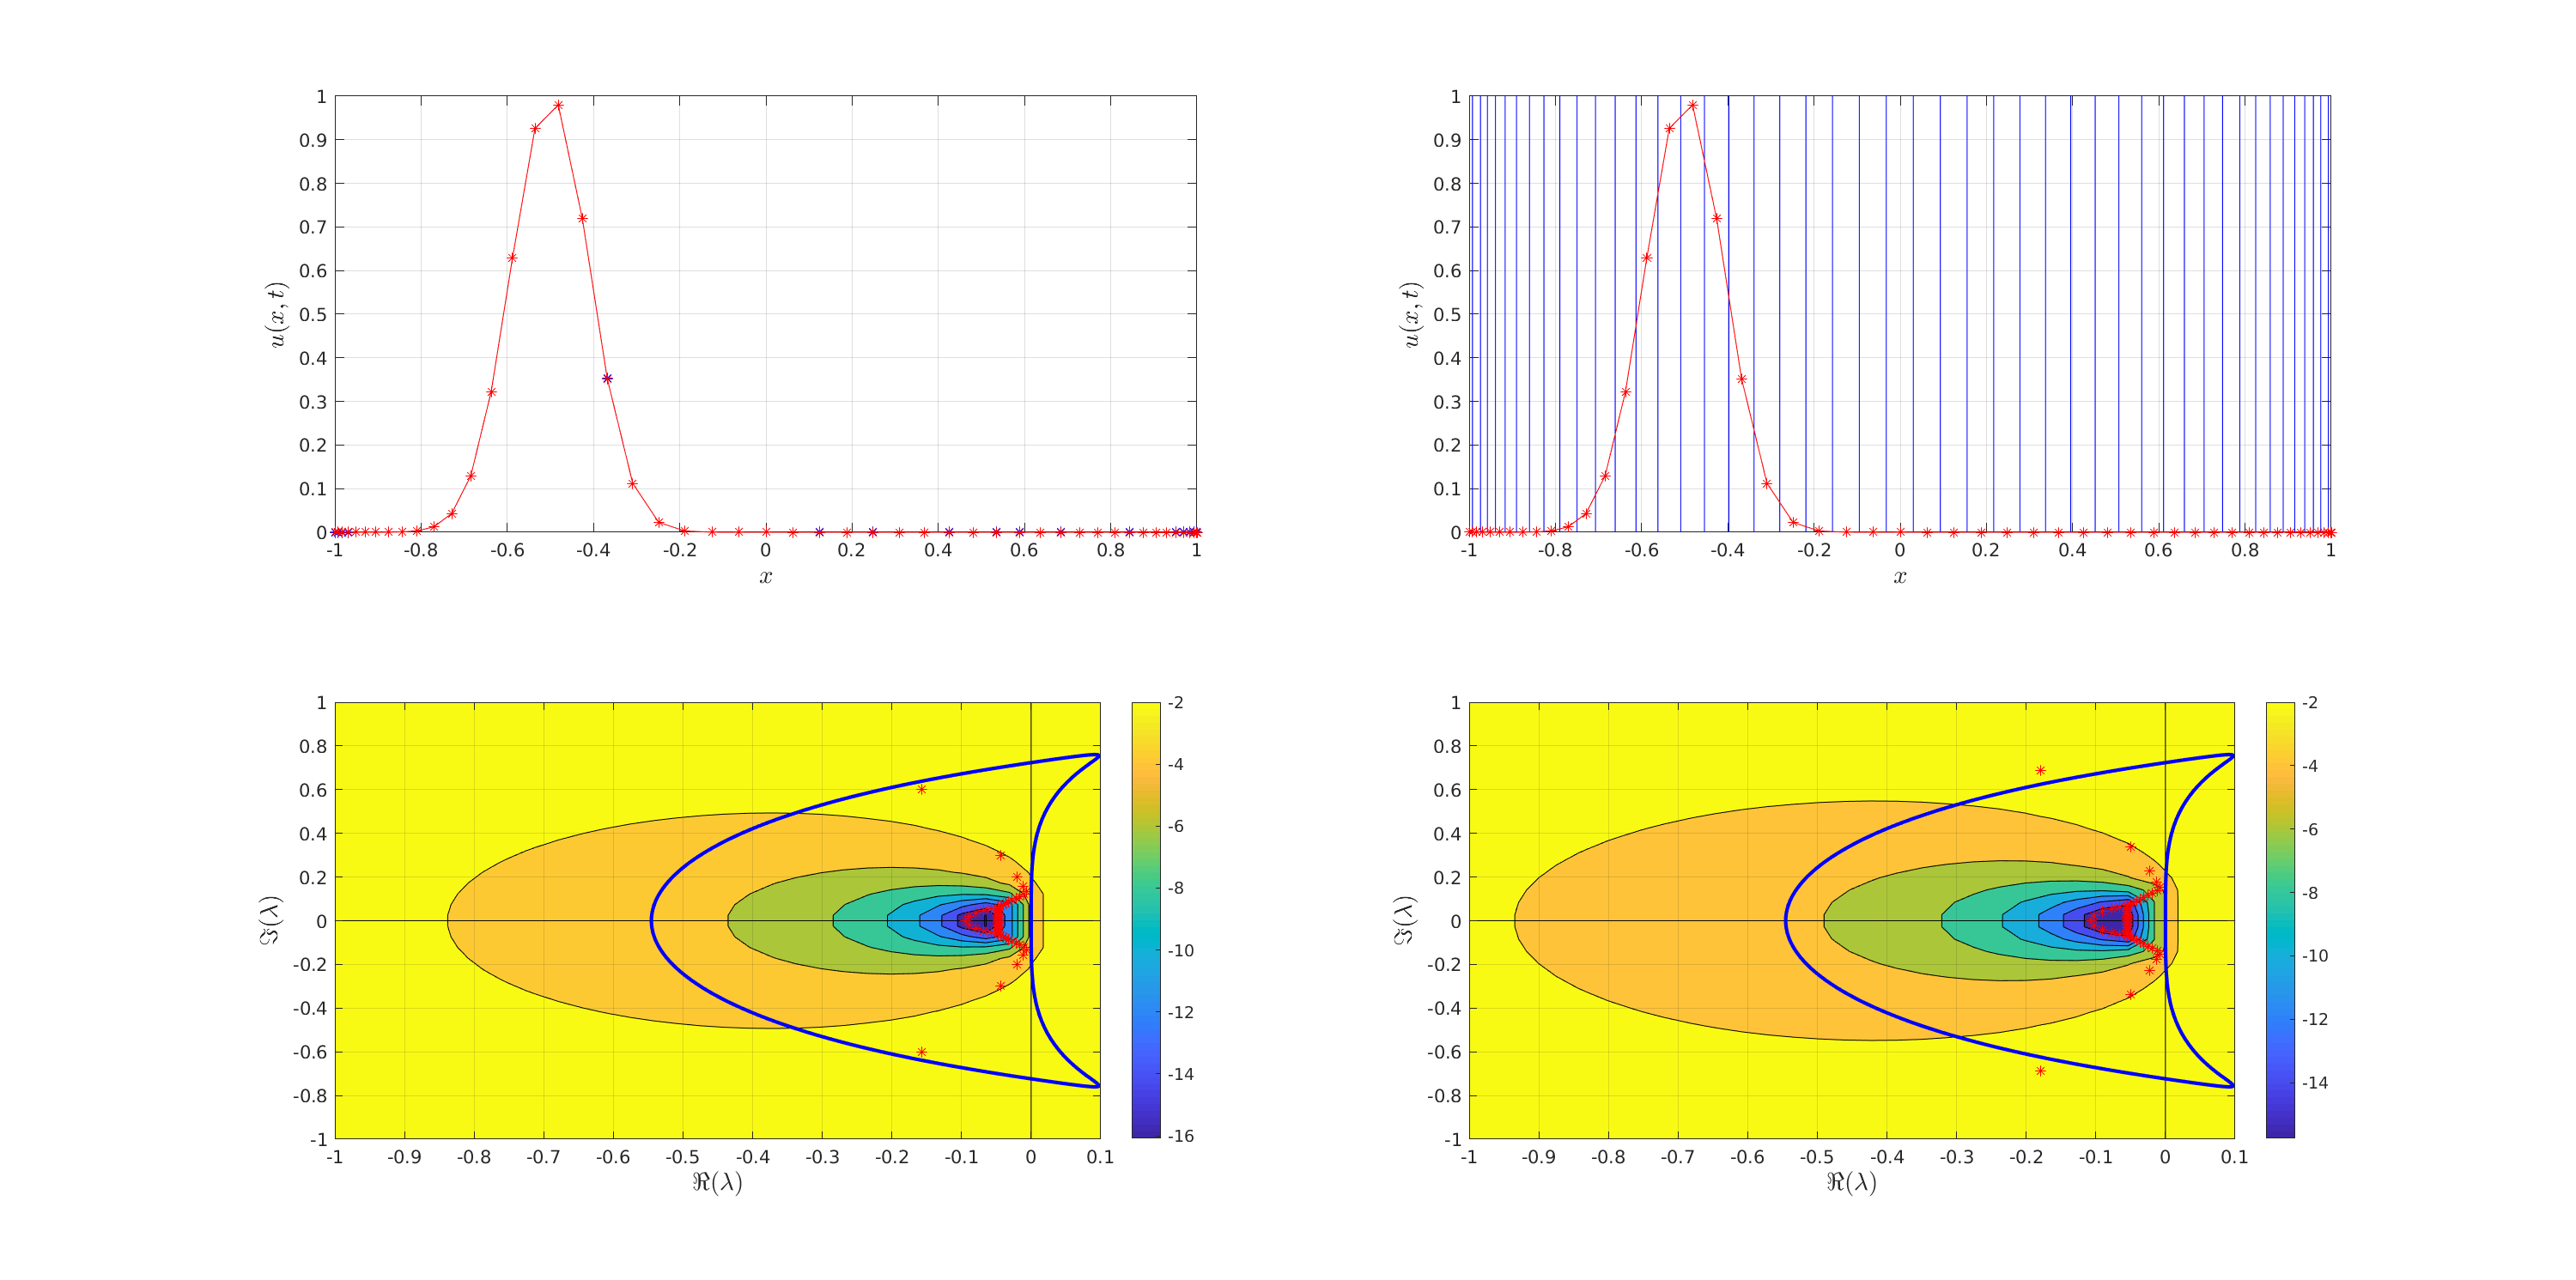
\includegraphics[scale=1.2]{P2.png}\caption{WRITE CAPTION.}
\end{figure}